\chapter{Calendar}
\section{Tasks identification from Work Breakdown Structure (WBS)}
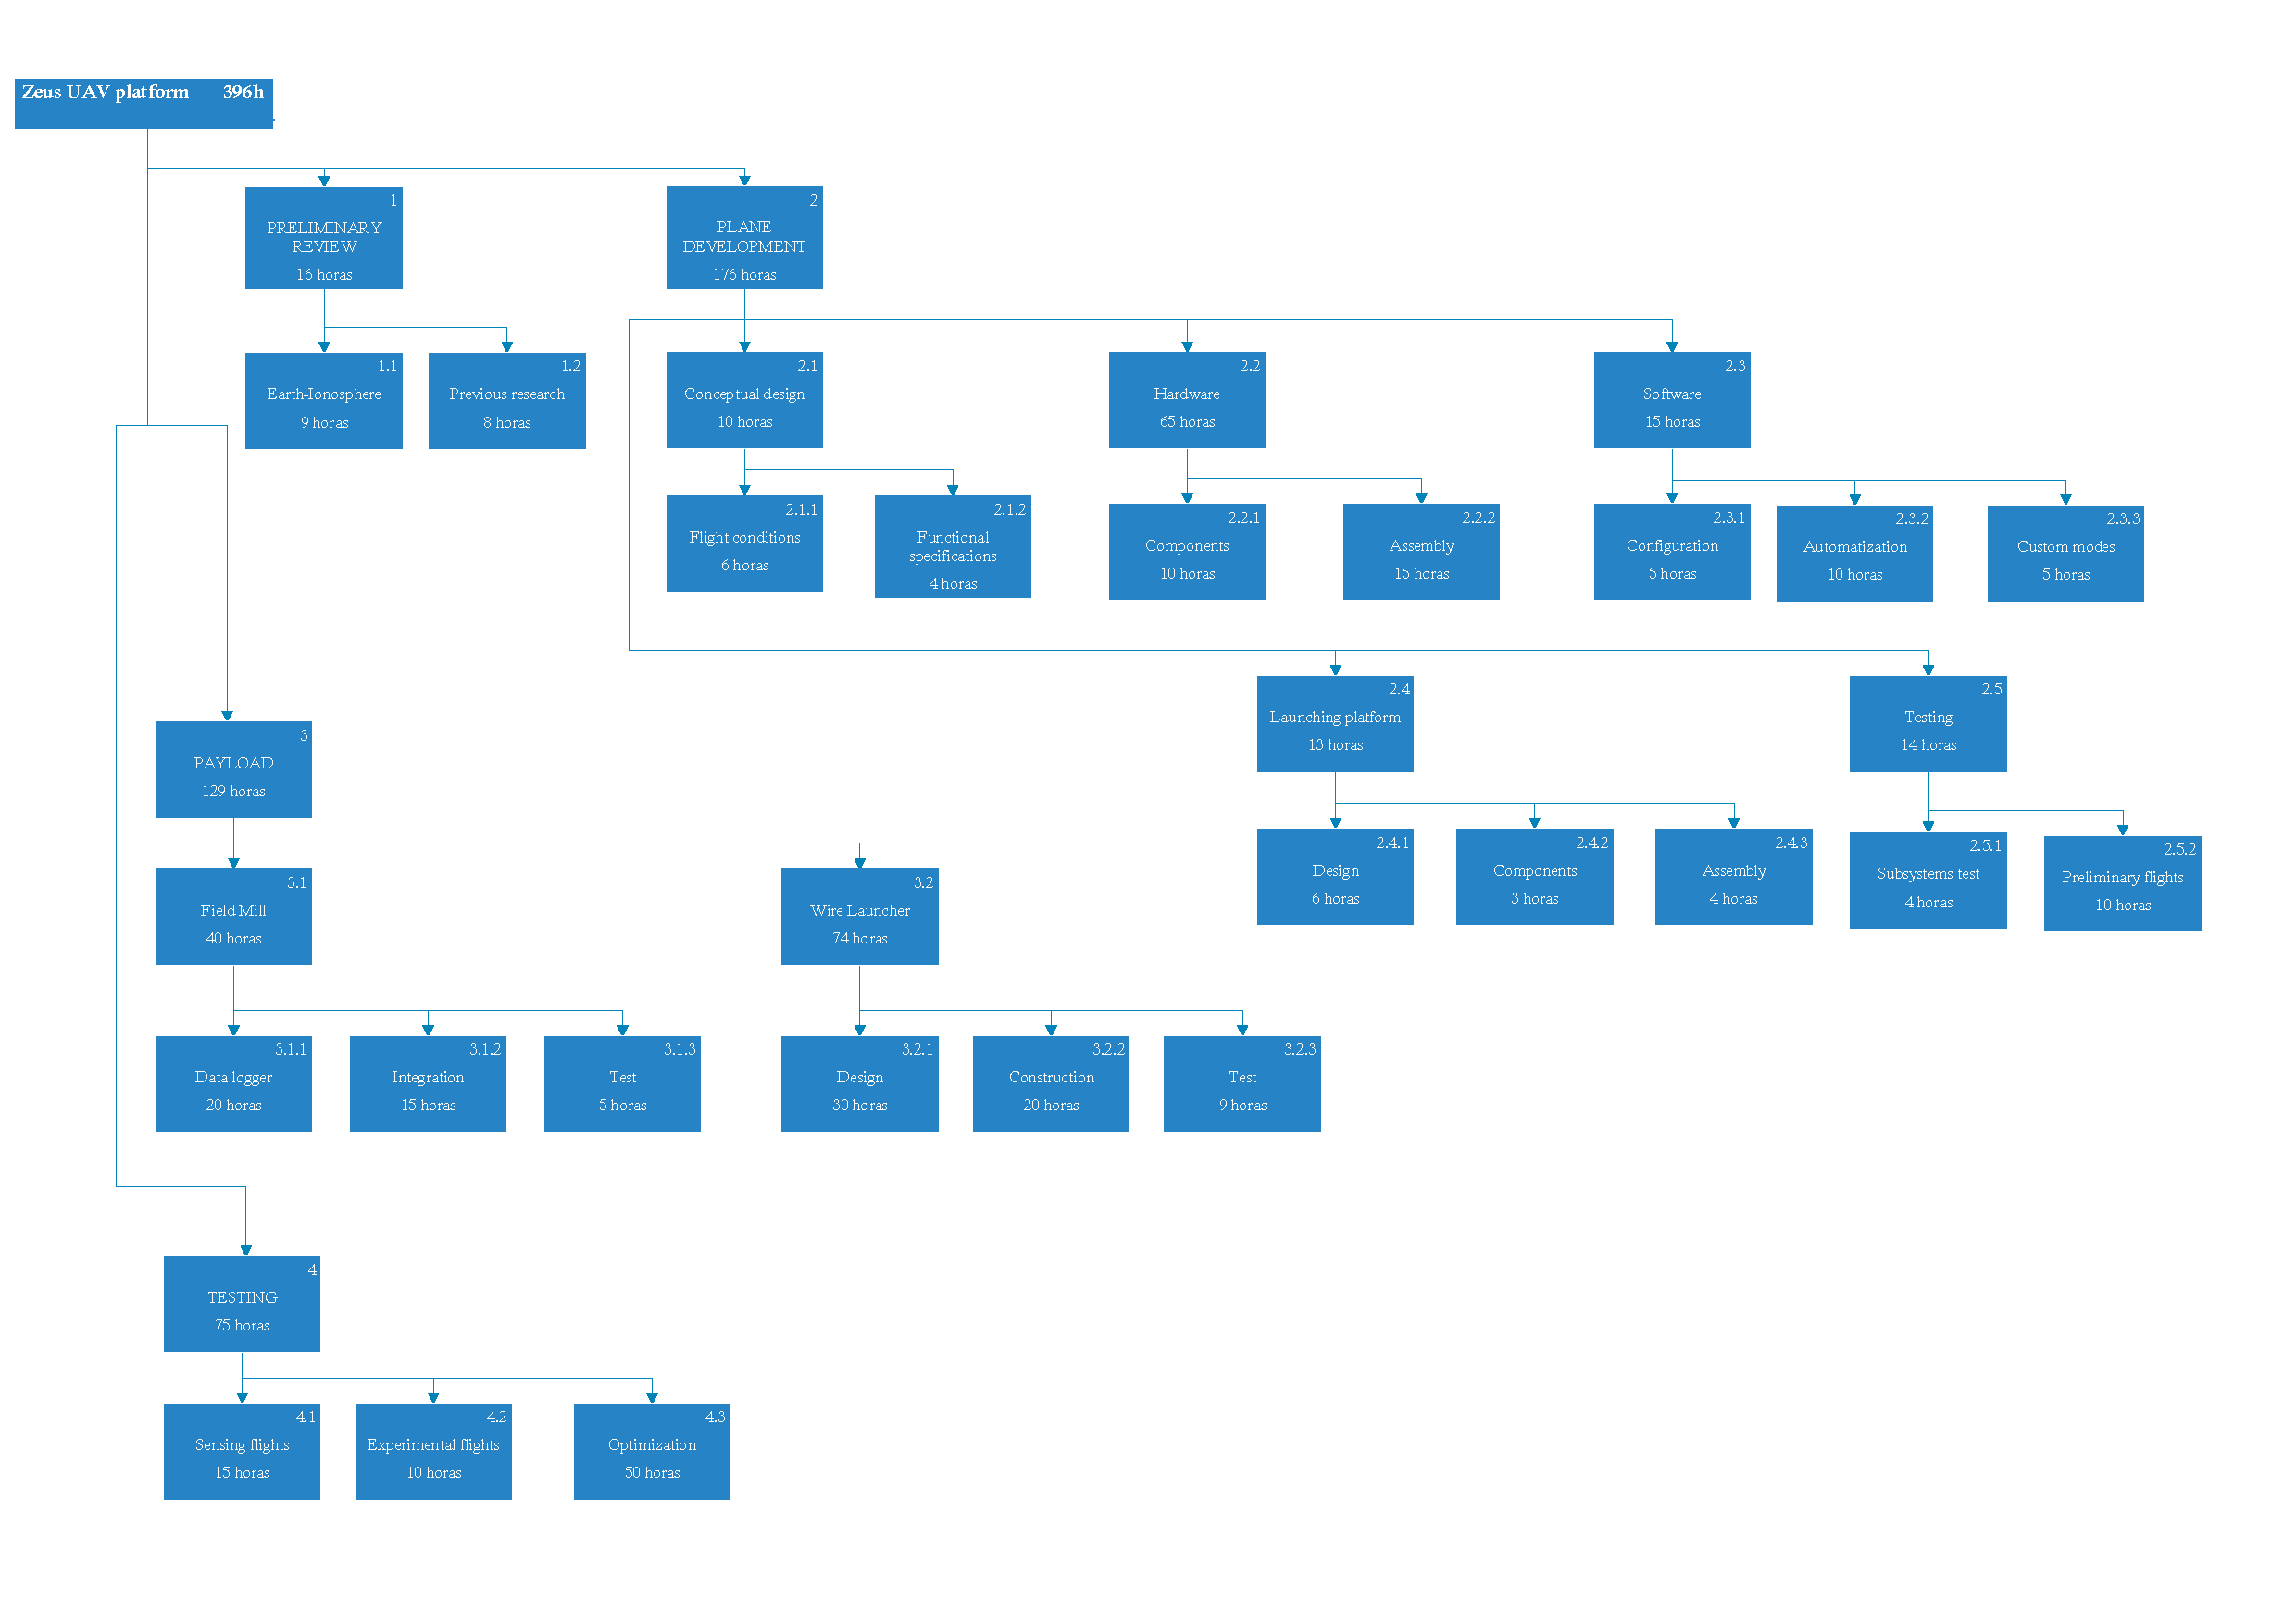
\includepdf[landscape=true]{./RAW/WBS}
\section{Tasks description}
\newcommand{\ra}[1]{\renewcommand{\arraystretch}{#1}}
\ra{1.3}
\begin{longtable}[htb]{@{}lll@{}}\toprule[3pt]
	%PRLIMINARY REVIEW
	\multicolumn{3}{c}{\textbf{\large 1. Preliminary review} }\\ \midrule[2pt]
		\textbf{ID} & \textbf{Work Package} &\textbf{Brief task description}\\ \midrule[1pt]
		1.1& Earth-Ionosphere& Review on earth-ionosphere main features and characteristics.\\
		1.2& Previous research& \begin{tabular}[c]{@{}l@{}}
			\begin{minipage}[t]{0.7\linewidth}
				State of the art on this field research.
			\end{minipage}
		\end{tabular} \\
	\midrule[2pt]
	%PLANE DEVELOPMENT
	\multicolumn{3}{c}{\textbf{\large 2. Plane development} }\\ \midrule[2pt]
	\textbf{ID} & \textbf{Work Package} &\textbf{Brief task description}\\ \midrule[1pt]
%Conceptual design
	2.1.1& Flight conditions& \begin{tabular}[c]{@{}l@{}}
		\begin{minipage}[t]{0.7\linewidth}
			Define under what flying conditions the UAV platform can operate. 
		\end{minipage}
	\end{tabular} \\
	2.1.2& Functional specifications& \begin{tabular}[c]{@{}l@{}}
		\begin{minipage}[t]{0.7\linewidth}
			Set and calculate the characteristic flying parameters that will determine when the UAV platform can operate. 
		\end{minipage}
	\end{tabular} \\

%Hardware
	2.2.1& Components& \begin{tabular}[c]{@{}l@{}}
		\begin{minipage}[t]{0.7\linewidth}
			Define and acquire all the necessary components to fully build de UAV.
		\end{minipage}
	\end{tabular} \\
	2.2.2& Assembly& \begin{tabular}[c]{@{}l@{}}
		\begin{minipage}[t]{0.7\linewidth}
			Build the UAV assembling all the defined components.
		\end{minipage}
	\end{tabular} \\
%Software
	2.3.1& Configuration& \begin{tabular}[c]{@{}l@{}}
		\begin{minipage}[t]{0.7\linewidth}
			Load and  configuration of the flying controller main software. 
		\end{minipage}
	\end{tabular} \\
	2.3.2& Automation& \begin{tabular}[c]{@{}l@{}}
		\begin{minipage}[t]{0.7\linewidth}
			Implement automatic flying and navigation modes for the UAV platform.
		\end{minipage}
	\end{tabular} \\
	2.3.3& Custom modes& \begin{tabular}[c]{@{}l@{}}
		\begin{minipage}[t]{0.7\linewidth}
			Adapt and create main UAV software modes which fits on the mission requirements.
		\end{minipage}
	\end{tabular} \\
%Launching platform
	2.4.1.& Design& \begin{tabular}[c]{@{}l@{}}
		\begin{minipage}[t]{0.7\linewidth}
			Design the launching platform including the calculations for achieving the desired UAV performance at Take Off.
		\end{minipage}
	\end{tabular} \\
	2.4.2.& Components& \begin{tabular}[c]{@{}l@{}}
		\begin{minipage}[t]{0.7\linewidth}
			Define all the necessary components to fully build the launching platform.
		\end{minipage}
	\end{tabular} \\
	2.4.3.& Assembly& \begin{tabular}[c]{@{}l@{}}
		\begin{minipage}[t]{0.7\linewidth}
			Build the UAV launching platform assembling the previous acquired components. 
		\end{minipage}
	\end{tabular} \\
%Testing
	2.5.1.& Subsystems test& \begin{tabular}[c]{@{}l@{}}
		\begin{minipage}[t]{0.7\linewidth}
			Test the correct operation of each plane subsystem.
		\end{minipage}
	\end{tabular} \\
	2.5.2.& Preliminary flights& \begin{tabular}[c]{@{}l@{}}
		\begin{minipage}[t]{0.7\linewidth}
			Perform the firsts flights in order to optimize the UAV operation.
		\end{minipage}
	\end{tabular} \\
	\midrule[2pt]
	%PAYLOAD
\multicolumn{3}{c}{\textbf{\large 3.Payload} }\\ \midrule[2pt]
\textbf{ID} & \textbf{Work Package} &\textbf{Brief task description}\\ \midrule[1pt]
%Field Mill
	3.1.1& Data logger& \begin{tabular}[c]{@{}l@{}}
		\begin{minipage}[t]{0.7\linewidth}
			Create a data logger making use of \textit{Arduino} like platform to store Field Mill readings.
		\end{minipage}
	\end{tabular} \\
	3.1.2& Integration& \begin{tabular}[c]{@{}l@{}}
		\begin{minipage}[t]{0.7\linewidth}
			Adapt the Field Mill and data logger system to the UAV platform payload bay.
		\end{minipage}
	\end{tabular} \\
	3.1.3& Test& \begin{tabular}[c]{@{}l@{}}
		\begin{minipage}[t]{0.7\linewidth}
			Test Field Mill performance as a UAV payload and calibrate the readings. 
		\end{minipage}
	\end{tabular} \\
%Wire launcher
	3.2.1& Design& \begin{tabular}[c]{@{}l@{}}
		\begin{minipage}[t]{0.7\linewidth}
			Conceive a wire launcher mechanism and design it.
		\end{minipage}
	\end{tabular} \\
	3.2.2& Construction& \begin{tabular}[c]{@{}l@{}}
		\begin{minipage}[t]{0.7\linewidth}
			Build the wire launcher mechanism previously conceived. 
		\end{minipage}
	\end{tabular} \\
	3.2.3& Test& \begin{tabular}[c]{@{}l@{}}
		\begin{minipage}[t]{0.7\linewidth}
			Test the performance of the mechanism until is suitable for the mission requirements.
		\end{minipage}
	\end{tabular} \\
%TESTING
	\midrule[2pt]
\multicolumn{3}{c}{\textbf{\large 4. Testing} }\\ \midrule[2pt]
\textbf{ID} & \textbf{Work Package} &\textbf{Brief task description}\\ \midrule[1pt]
	4.1& Sensing flights& \begin{tabular}[c]{@{}l@{}}
		\begin{minipage}[t]{0.7\linewidth}
			Preliminary flights to test the correction of the data acquired by the sensors.
		\end{minipage}
	\end{tabular} \\
	4.2& Experimental flights& \begin{tabular}[c]{@{}l@{}}
		\begin{minipage}[t]{0.7\linewidth}
			Real mission oriented flights. Real measurements will be done in order to study the atmosphere electricity.
		\end{minipage}
	\end{tabular} \\
	4.3& Optimization& \begin{tabular}[c]{@{}l@{}}
		\begin{minipage}[t]{0.7\linewidth}
			Based on the mission results and UAV platform performance, some features will be upgraded. 
		\end{minipage}
	\end{tabular} \\
%MILESTONES
\midrule[2pt]
\multicolumn{3}{c}{\textbf{\large Milestones} }\\ \midrule[2pt]
\textbf{ID} & \textbf{Work Package} &\textbf{Brief task description}\\ \midrule[1pt]
	5& START& \begin{tabular}[c]{@{}l@{}}
		\begin{minipage}[t]{0.7\linewidth}
			Project scheduled start 06/02/2017.
		\end{minipage}
	\end{tabular} \\
	6& Components arrival& \begin{tabular}[c]{@{}l@{}}
		\begin{minipage}[t]{0.7\linewidth}
			UAV platform scheduled components arrival 28/02/2017.
		\end{minipage}
	\end{tabular} \\
	7& END& \begin{tabular}[c]{@{}l@{}}
		\begin{minipage}[t]{0.7\linewidth}
			Scheduled project end 20/06/2017.
		\end{minipage}
	\end{tabular} \\
		\bottomrule[3pt]
	\caption{Tasks description}
\end{longtable}

\clearpage
\section{Tasks interdependency relationships}
\begin{longtable}[htb]{@{}llll@{}}\toprule[3pt]

%PRELIMINARY REVIEW
\multicolumn{4}{c}{\textbf{\large 1. Preliminary review} }\\ \midrule[2pt]
\textbf{ID} & \textbf{Work Package} &\textbf{Time (h)} &\textbf{Prelations}\\ \midrule[1pt]
	1.1& Earth-Ionosphere& 9 &BB-5\\
	1.2& Previous research& 8 & BF-1.1\\
	\midrule[2pt]
%PLANE DEVELOPMENT
\multicolumn{4}{c}{\textbf{\large 2. Plane development} }\\ \midrule[2pt]
\textbf{ID} & \textbf{Work Package} &\textbf{Time (h)} &\textbf{Prelations}\\ \midrule[1pt]
%Conceptual design
	2.1.1& Flight conditions& 6& \\
	2.1.2& Functional specifications& 4&BF-2.1.1 \\
%Hardware
	2.2.1& Components& 10&BF-2.1\\
	2.2.2& Assembly& 15& BF-3.1, 6\\
%Software
	2.3.1& Configuration& 5&BF-2.2.2, 3.2.1\\
	2.3.2& Automation& 10&BB-2.3.1\\
	2.3.3& Custom modes& 5&BF-2.3.2 \\
%Launching platform
	2.4.1.& Design& 6&BF-3.2\\
	2.4.2.& Components& 3&BF-2.4.1\\
	2.4.3.& Assembly& 4&BF-2.4.2\\
%Testing
	2.5.1.& Subsystems test& 4&BF-2.2, 2.3, 2.4\\
	2.5.2.& Preliminary flights& 10&BF-2.5.1\\
	\midrule[2pt]
%PAYLOAD
\multicolumn{4}{c}{\textbf{\large 3.Payload} }\\ \midrule[2pt]
\textbf{ID} & \textbf{Work Package} &\textbf{Time (h)} &\textbf{Prelations}\\ \midrule[1pt]
%Field Mill
	3.1.1& Data logger& 20&BF-2.2.1\\
	3.1.2& Integration& 15&BF-3.1.1\\
	3.1.3& Test& 5&3.1.2\\
%Wire launcher
	3.2.1& Design& 30&BF-2.2.2, 3.1\\
	3.2.2& Construction& 20&BF-2.3, 3.2.1\\
	3.2.3& Test& 5&BF-3.2.2\\
	& & & \\
%TESTING
\midrule[2pt]
\multicolumn{4}{c}{\textbf{\large 4. Testing} }\\ \midrule[2pt]
\textbf{ID} & \textbf{Work Package} &\textbf{Time (h)} &\textbf{Prelations}\\ \midrule[1pt]
	4.1& Sensing flights& 15& BF-2, 3\\
	4.2& Experimental flights& 10& BF-4.1\\
	4.3& Optimization& 50&BF-4.2 \\
\bottomrule[3pt]
\caption{Tasks relationships}
\end{longtable}
\section{Project Gantt diagram}
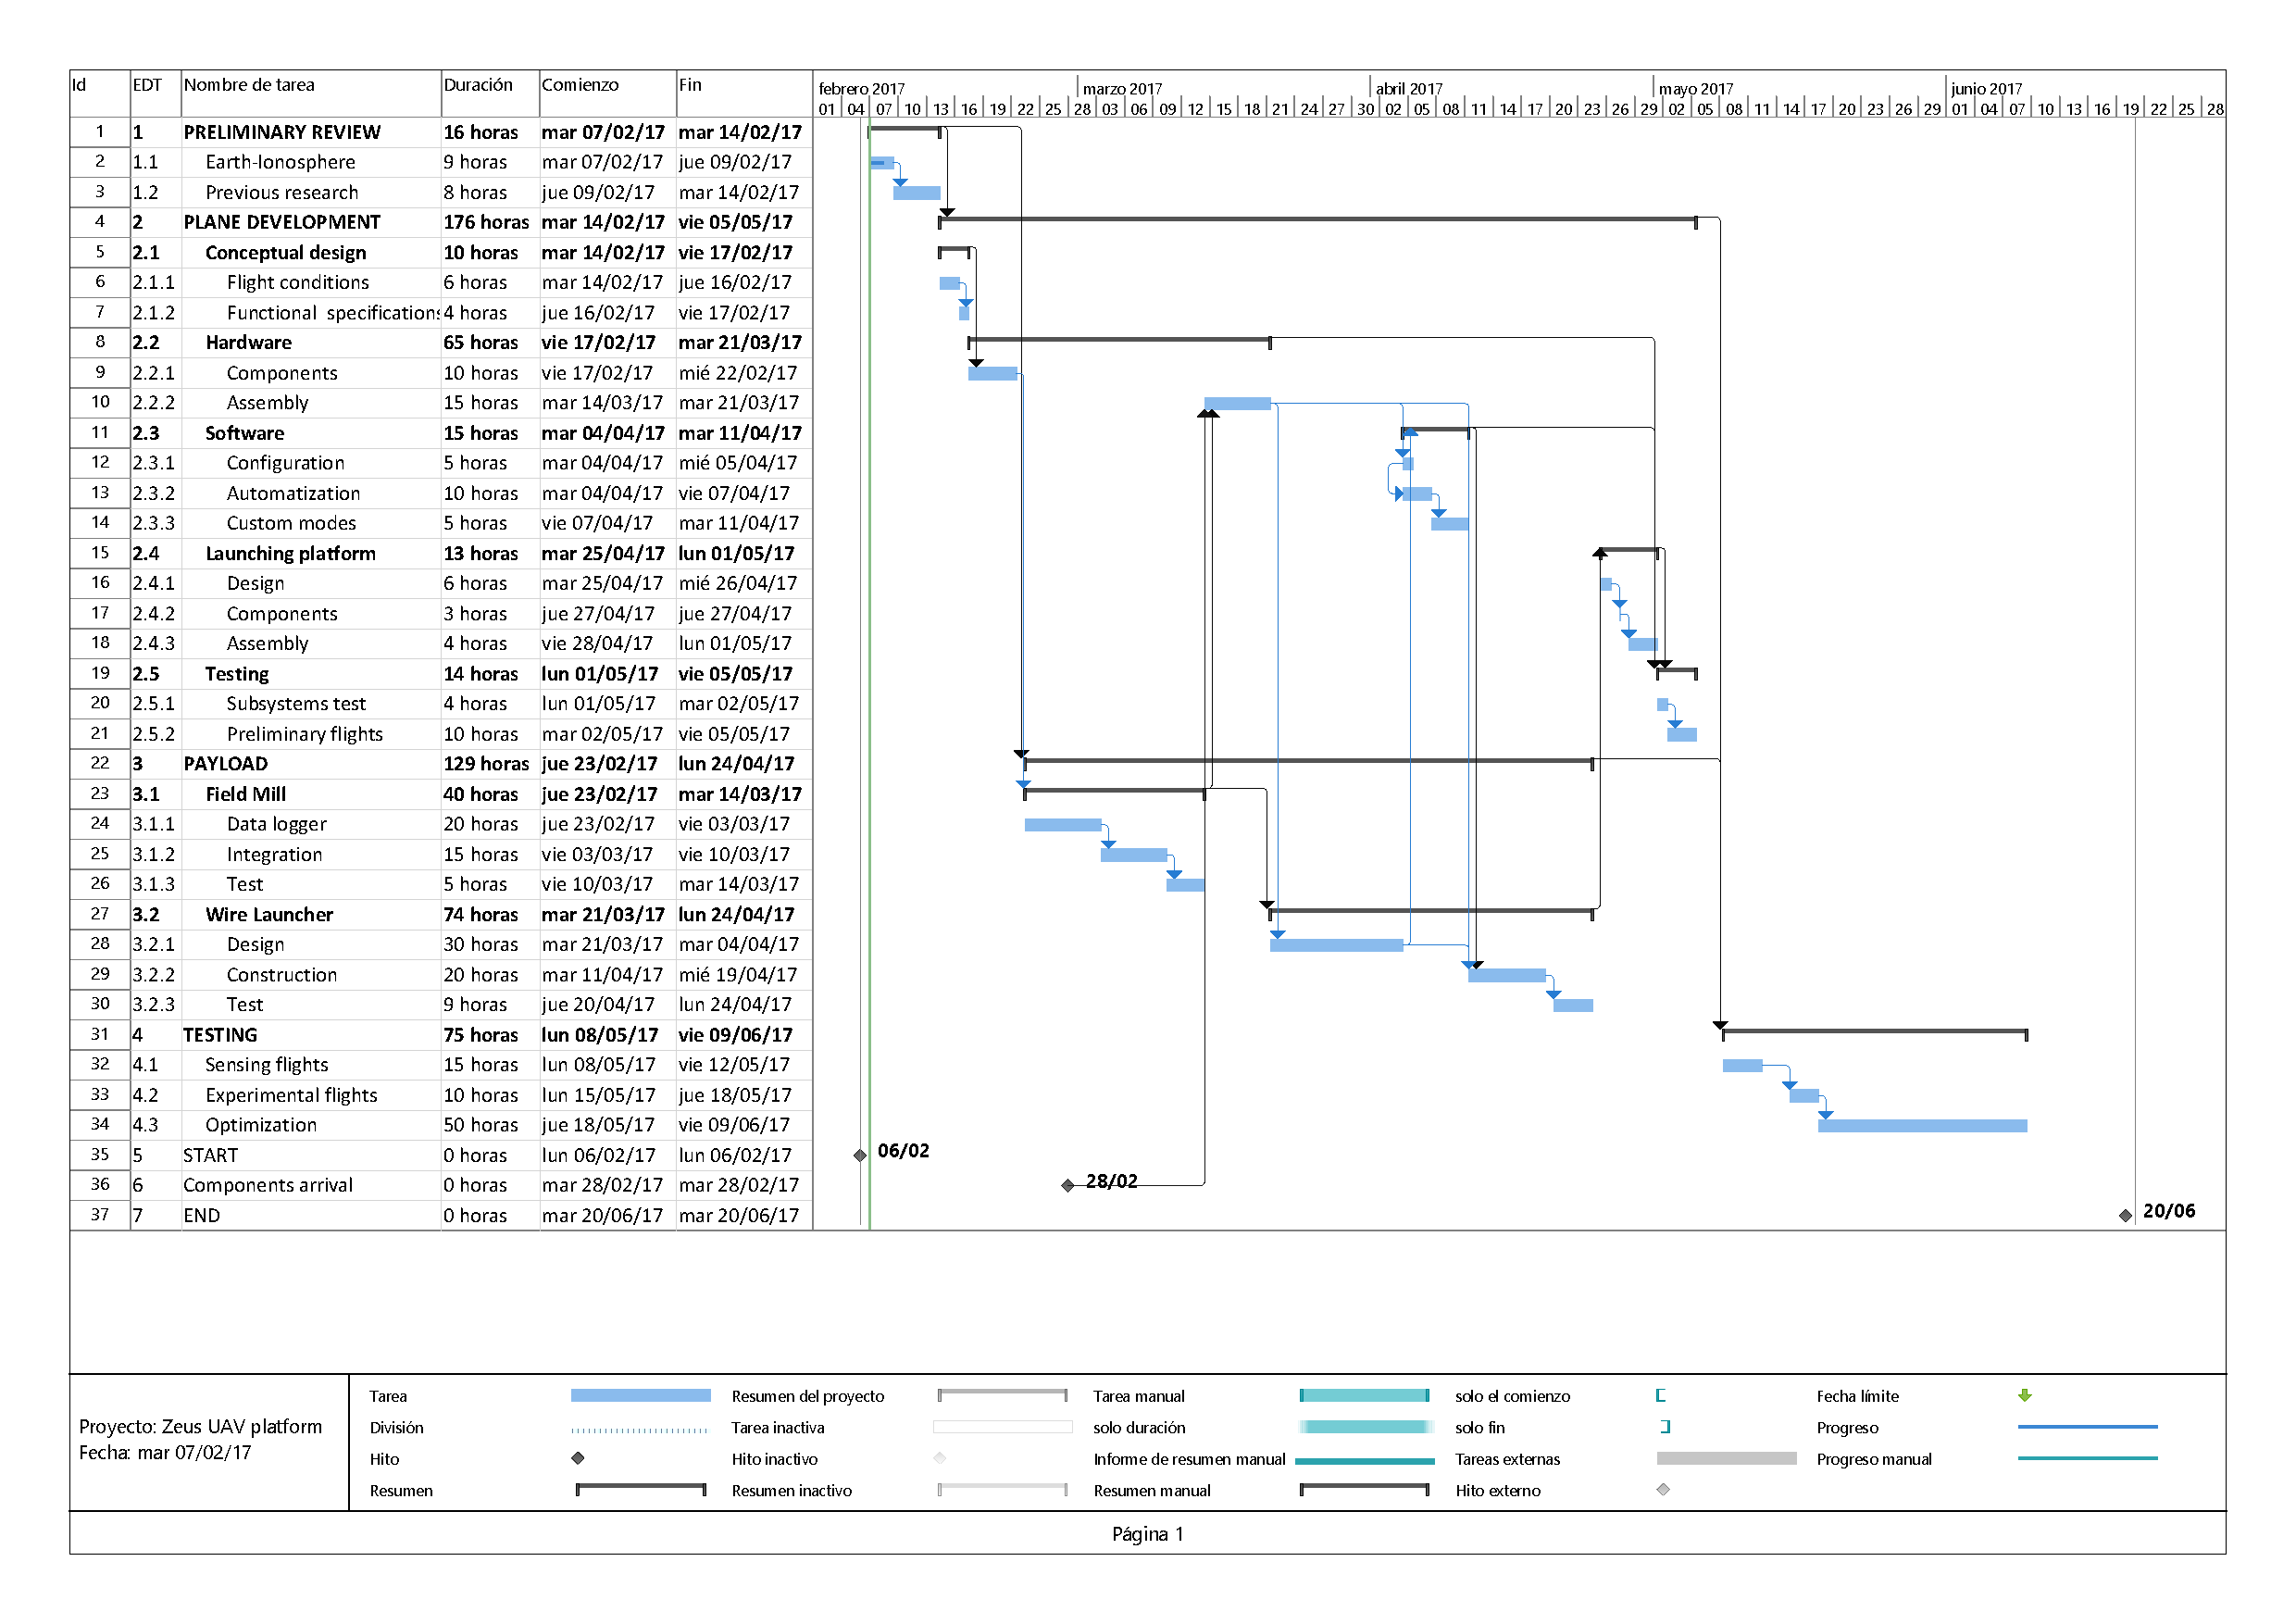
\includepdf[landscape=true]{./RAW/GANTT}